\documentclass[10pt]{article}

\usepackage{titlesec}

% Section titles and subsection titles settings
\titleformat{\section}{\normalfont\large\bfseries}{\thesection}{2em}{}
\titlespacing*{\section}{0pt}{1\baselineskip}{1\baselineskip}
\titleformat{\subsection}{\normalfont\small\bfseries}{\thesubsection}{1em}{}[]
\titlespacing{\subsection}{0pt}{1\baselineskip}{1\baselineskip}


% Font
\usepackage[T1]{fontenc}
\usepackage[scaled]{uarial}
\renewcommand*\familydefault{\sfdefault}

% Page layout
\usepackage[a4paper,margin=0.9in]{geometry}
\usepackage{wrapfig}
\setlength{\intextsep}{10pt} % Adjust the vertical space
\setlength{\columnsep}{10pt} % Adjust the horizontal space

% Math
\usepackage{mathptmx}
\usepackage{amsfonts}

% Fonts
\usepackage{fontspec}

% Hyperlinks
\usepackage{hyperref}

% Colors
\usepackage{xcolor}

% Tables
\usepackage{booktabs}
\usepackage{siunitx}

% Figures
\usepackage{graphicx}
\usepackage{caption}
\captionsetup[figure]{skip=2pt} 



% Title and Author information
\title{
    \vspace{-2cm}Classification Model Generalization on NinaPro Dataset
}
\author{
    \vspace{0.2cm}Antea Ceko, Chiara Billi, Irene Vardabasso, Ludek Cizinsky, Lou Houngbedji \\
    \vspace{0.2cm} \normalsize{Ecole Polytechnique Fédérale de Lausanne, Switzerland}
}

\date{\today}

\begin{document}
\maketitle

\section{Introduction}
In recent years, machine learning-based approaches have demonstrated success across various fields,  including the medical domain. 
This project focuses on evaluating different classification models capable of predicting the type of movement executed by a patient based on surface electromyography (sEMG) signals recorded 
from the patient's forearm. The dataset utilized for this project is the NinaPro dataset DB1 \cite{ninapro}, 
comprising sEMG signals recorded from 27 patients while performing various hand movements.

\section{Data and Preprocessing Steps}
The sEMG dataset under consideration was acquired using a setup featuring 10 electrodes. 
This dataset comprises 10 repetitions of 52 distinct movements. 
Participants were presented with video prompts displayed on a laptop screen, 
guiding them to replicate the specified movements. Each repetition spanned a duration of 
5 seconds, followed by a 3-second rest interval. The experimental protocol encompassed three distinct exercise categories. 
Firstly, participants engaged in \textit{fundamental finger movements}. 
Subsequently, they undertook activities involving \textit{isometric and isotonic hand configurations}, 
coupled with basic wrist motions. Lastly, the participants performed exercises related to \textit{grasping and functional movements} \cite{ninapro}.

\textbf{Preprocessing Strategy.} In our work, we concentrated on the initial category of movements, encompassing 12 distinct hand gestures and totaling seven and a half hours of sEMG data. 
The alignment between the sEMG signals and corresponding labels was performed by the authors of the NinaPro dataset. 
Addressing potential disparities between subject movements and software stimuli, the authors employed a generalized likelihood ratio algorithm to 
correct inaccurate movement labels \cite{ninapro}.

It is important to note that the sEMG signals had already undergone preprocessing by the electrode manufacturer, 
utilizing a Root Mean Square (RMS) filter. Therefore, we adapted the approach taken by Atzori et al. \cite{ninapro}, i.e., 
we implemented a low-pass filter on the sEMG signals, with a cutoff frequency of $5 Hz$, employing a zero-phase second-order Butterworth filter.

\begin{figure}[ht]
\centering
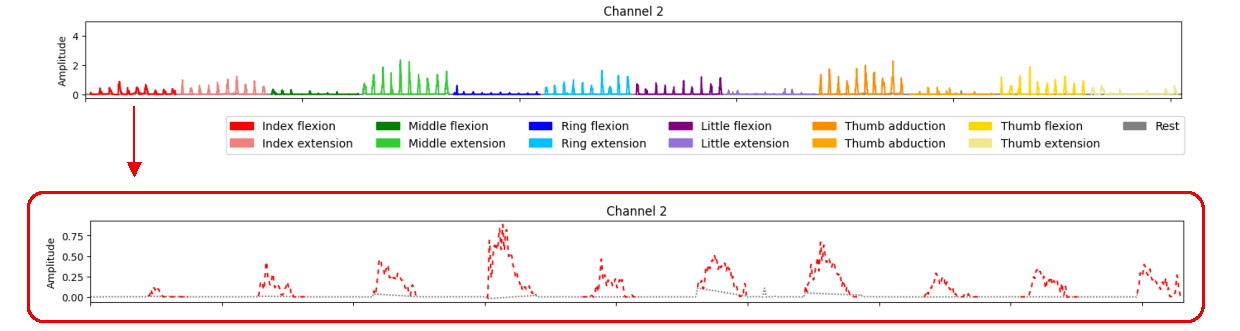
\includegraphics[width=1\textwidth]{../figures/preprocessing.pdf}
\caption{The first plot illustrates the preprocessed sEMG signal for the initial subject across one of the 10 channels. 
The subsequent plot provides a detailed examination of the \texttt{Index flexion} finger movement and its 10 repetitions.}
\label{fig:preprocessing}
\end{figure}

\textbf{Data Splits and Windowing.} In Figure \ref{fig:preprocessing}, sEMG signals are recorded in 10 repetitions, displaying amplitude variations. 
To ensure representative training, validation, and test sets, each split includes repetitions from both the trial's start and end. 
The training split comprises the 1st, 3rd, 5th, 7th, and 9th repetitions; 
the validation split includes the 2nd, 4th, and 8th repetitions, 
and the test split involves the 6th and 10th repetitions. 
This approach ensures that the model is trained and evaluated on the representative data. 
Notably, since each repetition of a given stimuli is associated with the rest period,
we assigned the rest period to the same split as the corresponding repetition.

\begin{figure}[ht]
    \centering
    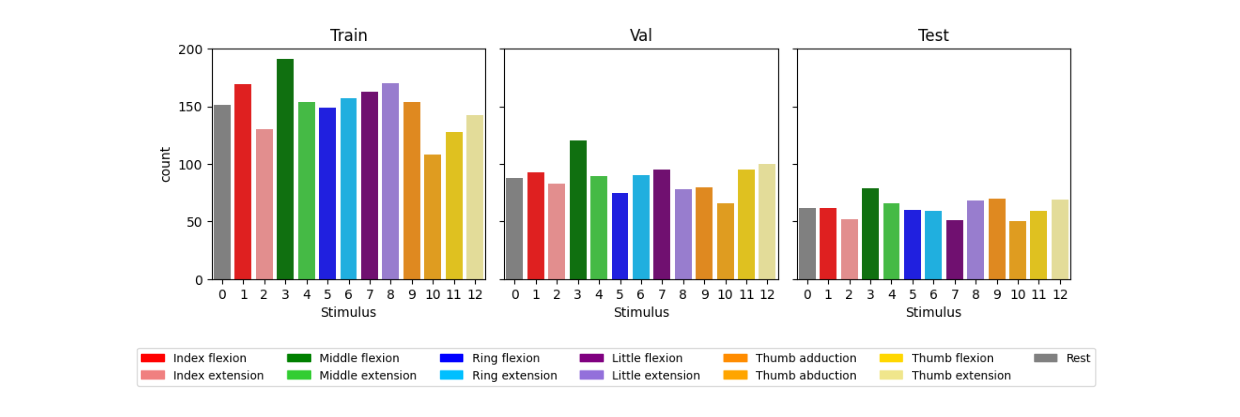
\includegraphics[width=1\textwidth]{../figures/downsampling.pdf}
    \caption{Distribution of the stimuli classes accross splits for the 17th subject.}
    \label{fig:downsampling}
\end{figure}

For each split and subject, we performed windowing with a window size of $500$ ms and a stride of $100$ ms. 
This choice balances capturing movement information for effective classification and considering temporal dynamics without 
excessive computational cost. With a sampling frequency of $100$ Hz, the chosen stride yields a sample for every time point. 
Importantly, each window's label is assigned based on the majority label. The windowing technique introduces a notable class imbalance—40\% stimuli classes and 60\% rest periods. 
To mitigate bias towards the rest period, we applied downsampling, equalizing the rest period samples to the average number per class, 
as depicted in Figure \ref{fig:downsampling}.

\textbf{Feature Extraction}. For each window, we decided to extract both time and frequency domain features. For time, we extracted 
Mean Absolute Value (\texttt{MAV}), Maximum Absolute Value (\texttt{MaxAV}), Wavelength (\texttt{WL}), Standard Deviation (\texttt{STD}), and Root Mean Square (\texttt{RMS}). 
Additional, in the frequency domain, we considered Mean Power, Total Power, Mean Frequency, Median Frequency, and Peak Frequency. Prior to inputting the features to the model,
we applied standard scaling to ensure that all features have zero mean and unit variance. 

\begin{figure}[ht]
    \centering
    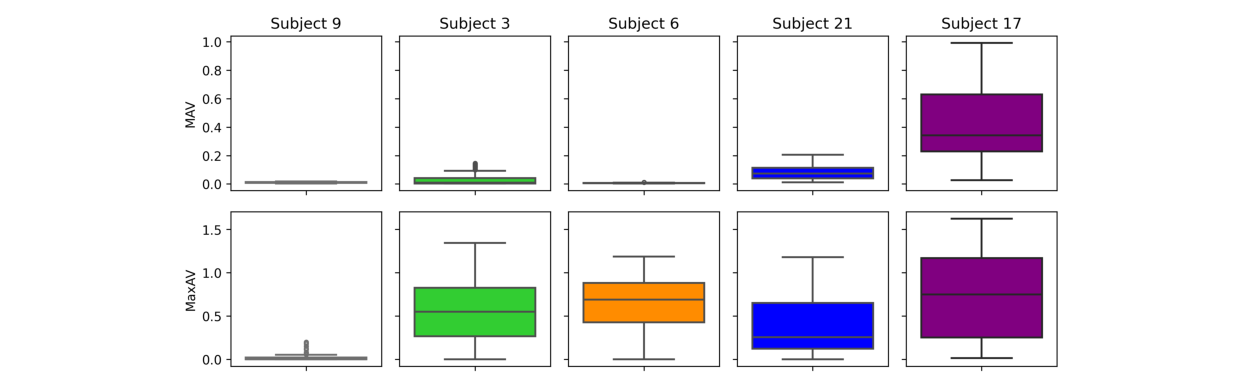
\includegraphics[width=1\textwidth]{../figures/inter_sub_var.pdf}
    \caption{Variability of selected features of Index Flexion stimuli, \texttt{MAV} and \texttt{MaxAV}, accross subjects. 
    The boxplot is showing median, 25th and 75th percentiles, and max-min of the features.}
    \label{fig:feat_var}
\end{figure}

The variability of selected features, specifically \texttt{MAV} and \texttt{MaxAV}, 
across subjects for Index Flexion stimuli is depicted in Figure \ref{fig:feat_var}. 
This visual representation highlights significant differences in the extracted time features among subjects. 
Possible explanations for these variations include differences in physiological factors such as muscle strength, anatomy, or motor control strategies.
This is a known challenge when working with sEMG data which has been recently tackled in various works 
via Deep Learning based methods \cite{dl2, dl1}. 

\section{Methods}
We start with the training and evaluation of a selected set of models on individual subjects, 
specifically Softmax Regression (\texttt{SR}), K-Nearest Neighbors (\texttt{KNN}), and Random Forest (\texttt{RF}). 
Through an extensive grid search, we determine optimal hyper-parameters for each model. 
This phase of the experiment aims to validate our foundational hypothesis: that the chosen models exhibit the capability to generalize 
from a subject's training data to the corresponding unseen test data. 
Furthermore, we investigate whether models trained on individual subjects leverage similar features. For that, we compute the permutation
feature importance which is a metric that indicates how much the model's performance decreases when a given feature is randomly shuffled. 
In the subsequent phase, subjects are randomly divided into training ($20$) and test ($7$) sets. 
We identify the best-performing model from the previous step and train it 
on a chosen subset of training subjects, varying in size ($K$). For each $K$, we repeat the training 
and evaluation process five times, reporting the mean along with a 95\% confidence interval (CI) 
for the test accuracy. This phase of the experiment aims to validate our second hypothesis: the model's generalization 
performance improves with an increasing number of training subjects.

\section{Results and Discussion}
\begin{table}[ht]
    \centering
    \begin{tabular}{llr}
        \toprule
        \textbf{Model} & \textbf{Best Configuration Accross Subjects} & \textbf{Test Acc $\pm$ 95CI} \\
        \midrule
        Random Forest & \texttt{MaxDepth=}15,\texttt{NofEstimators=}300, \texttt{MaxFeat=}\texttt{sqrt} & $\mathbf{0.82 \pm0.04}$ \\
        Softmax Regression & \texttt{Loss=hinge}, \texttt{Penalty=L1}, \texttt{Alpha=}=$1e^{-4}$, \texttt{MaxIter=}270 &  $0.74 \pm0.05$ \\
        K-Nearest Neighbors & \texttt{NofNeighbors=}2, \texttt{Weights=distance} &  $0.65 \pm0.05$ \\
        \bottomrule
    \end{tabular}
    \caption{Results of training and evaluating the chosen models on individual subjects. 
    The best configuration for each model is a mean of the numeric hyper-parameters, 
    and the most frequent value for the categorical hyper-parameters.}
    \label{tab:results1}
\end{table}

Table \ref{tab:results1} shows that the best-performing model is by far \texttt{RF}, 
achieving 82\% test accuracy. This is comparable to the performance reported 
by Atzori et al. \cite{ninapro}. However, our task only consists of 12 movements 
instead of 52. Interestingly, we were able to achieve a solid baseline performance even 
with our linear model (\texttt{SR}). This suggests the high quality of the extracted features, 
making the prediction task easier for the model. Last but not least, while it is important, 
in general, to consider regularization, for our models, it played only a minor role given the low 
values of the regularization hyper-parameters.

\begin{figure}[ht]
    \centering
    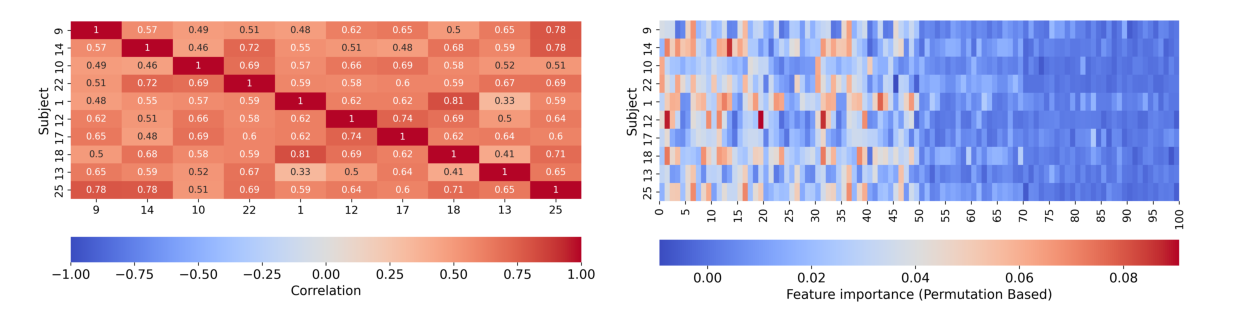
\includegraphics[width=1\textwidth]{../figures/fig_feat_imp.pdf}
    \caption{Both figures depict the feature permutation importance for the \texttt{SR} model. 
    The left plot illustrates the correlation among individual subjects' feature importance, 
    while the right plot showcases the significance of each feature for every subject}
    \label{fig:feat_imp}
\end{figure}

Figure \ref{fig:feat_imp} indicates varying feature importance across subjects. The left plot suggests 
a relatively high correlation in feature ranking among subjects. 
However, the right plot reveals that the correlation is likely driven by the last 50 features, 
consistently ranked low by all subjects. In contrast, the first 50 features exhibit significant ranking variation. 
This aligns with Figure \ref{fig:feat_var}, illustrating variability in individual feature values across subjects. 
Consequently, it's expected that models trained on individual subjects utilize different features.

\begin{wrapfigure}[12]{r}{0.5\textwidth}
    \centering
    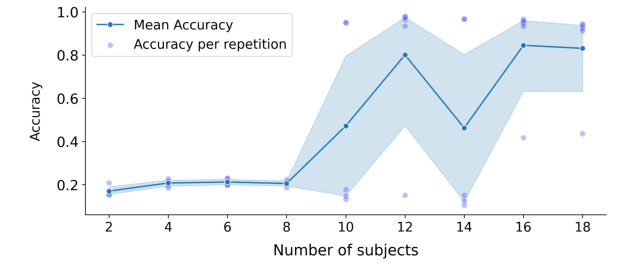
\includegraphics[width=0.5\textwidth]{../figures/fig_k_vs_perf.pdf}
    \caption{Test Accuracy of the \texttt{RF} model trained on different number of subjects.}
    \label{fig:k_vs_perf}
\end{wrapfigure}

Figure \ref{fig:k_vs_perf} shows the results of our second experiment. Compare to the first experiment,
the task is inherently more challenging since the model is trained on different set of subjects than the ones used for evaluation.
As the Figure \ref{fig:feat_var} shows, the subjects exhibit significant variability in the extracted features. Therefore,
it is expected that the more subjects are used for training, the better generalization performance the model should have.
Figure \ref{fig:k_vs_perf} confirms this hypothesis. Interestingly, the performance significantly improves when the model is trained on more than 10 subjects. 
However, it is crucial to consider the wide confidence interval, indicating the model's performance 
dependence on the similarity between training and test subjects.

\section{Conclusion}
In this project, we assessed the generalization of classification models on the NinaPro dataset DB1. 
Initially, we trained and evaluated models on individual subjects, achieving a competitive 81\% test accuracy with the \texttt{RF} model. 
Notably, models trained on individual subjects utilized distinct features. 
In the second part of the experiment, training on over 10 subjects significantly improved model performance. 
However, a wide confidence interval indicates performance dependency on the similarity between training and test subjects. 

\newpage
\bibliographystyle{abbrv}
\bibliography{references}

\end{document}